\documentclass[conference]{IEEEtran}
\IEEEoverridecommandlockouts
% The preceding line is only needed to identify funding in the first footnote. If that is unneeded, please comment it out.
\usepackage[utf8]{inputenc}

\usepackage{cite}
\usepackage{amsmath,amssymb,amsfonts}
\usepackage{algorithmic}
\usepackage{graphicx}
\usepackage{textcomp}
\usepackage{xcolor}
\usepackage{xspace}
\usepackage{paralist}
\usepackage{float}
\usepackage{booktabs}
\usepackage{hyperref}

\usepackage{flushend}

\def\BibTeX{{\rm B\kern-.05em{\sc i\kern-.025em b}\kern-.08em
    T\kern-.1667em\lower.7ex\hbox{E}\kern-.125emX}}
\begin{document}

\newcommand{\tool}{\textsc{SALVO}\xspace}
\newcommand{\challenge}{2021 IEEE Autonomous Driving AI Test Challenge\xspace}

\newboolean{showcomments}
\setboolean{showcomments}{false}         
%\setboolean{showcomments}{false} 
\ifthenelse{\boolean{showcomments}}
  {\newcommand{\nb}[2]{
  \fbox{\bfseries\sffamily\scriptsize#1}
     {\sf\small$\blacktriangleright$\textit{\textcolor{red}{#2}}$\blacktriangleleft$}
   }
  }
  {\newcommand{\nb}[2]{}
   \newcommand{\cvsversion}{}
  }

\newcommand\alessio[1]{\nb{Alessio}{#1}} 
\newcommand\vuong[1]{\nb{Vuong}{#1}} 
\newcommand\stefan[1]{\nb{Stefan}{#1}} 

%\title{\tool: Automated Generation of Diversified Tests for Self-driving Cars based on Photo-Realistic Maps}
\title{\tool: Automated Generation of Diversified Tests for Self-driving Cars from Existing Maps}



\author{
\IEEEauthorblockN{Vuong Nguyen}
\IEEEauthorblockA{\textit{University of Passau} \\
Passau, Germany \\
nguyen58@ads.uni-passau.de}
\and
\IEEEauthorblockN{Stefan Huber}
\IEEEauthorblockA{\textit{University of Passau} \\
Passau, Germany \\
stefan.huber.niedling@outlook.com}
\and
\IEEEauthorblockN{Alessio Gambi}
\IEEEauthorblockA{\textit{University of Passau} \\
Passau, Germany \\
alessio.gambi@uni-passau.de}
}

\maketitle

\begin{abstract}
Simulation-based tests are more cost-effective and less dangerous than field tests; hence, they are becoming the norm for thoroughly testing self-driving cars in virtual environments. High-quality simulation-based testing requires physically accurate computer simulations,  detailed and photo-realistic maps, and systematic approaches for generating tests. Moreover, since creating detailed maps is a manual process, they are expensive, and testers should avoid wasting such valuable resources, for example, by generating irrelevant test cases. To address those issues, we propose \tool a fully automated approach to identify quantifiably diverse and critical driving scenarios that can be instantiated on existing high-definition maps and implement them in an industrial driving simulator as executable test cases.
The evaluation of \tool in the context of the \challenge showed that it could analyze maps of different complexity and identify many critical driving scenarios in minutes. Furthermore, the tests \tool generated stressed a state-of-art self-driving car software in quantifiably diverse ways and exposed issues with its implementation.
\end{abstract}

 \begin{IEEEkeywords}
Test Case Generation, Autonomous Vehicles, Software-in-the-loop, Diversity, Feature Space
 \end{IEEEkeywords}

\section{Introduction and Motivation}
Self-driving cars promise to reduce traffic accidents \cite{peden2016status}, increase fuel efficiency~\cite{zamzuri2016current} and enhance comfort~\cite{harper2016estimating}.
Testing self-driving car software is laborious and challenging since self-driving car's development is still in an early stage, and there is a lack of standardized procedures and established approaches \cite{gambi2019generating}. Therefore, many researchers and organizations are currently investigating testing approaches to increase the quality of autonomous vehicles before they roam the thoroughfares.
%
Naturalistic field operational testing is a popular approach to validate and verify the safety of autonomous vehicles that leaves them free to drive on actual roads. However, as discussed by Kalra and Paddock~\cite{kalra2016driving}, this method is inefficient since relevant execution conditions (e.g., traffic situations that lead to traffic accidents) are hard to observe and ineffective as dangerous situations are impossible to recreate. Those, in turn, make limit the replicability of natural field operational tests' results ~\cite{hasenau2019virtual}. An alternative approach is virtual testing, also known as simulation-based testing, which uses computer simulations to generate diverse test cases to challenge the self-driving software involving traffic patterns and numerous virtual road conditions~\cite{hasenau2019virtual}. Virtual testing enables automated test execution and can expose problems in autonomous software, including perception, planning, and decision-making systems. However, it requires the availability of accurate geometrical models (e.g., 3D models with textures and material properties) to achieve photo-realism, i.e., to close the simulation-to-reality gap~\cite{9207173}, and detailed road maps. Consequently, cartography is an essential building block to conduct thorough virtual testing of autonomous vehicles~\cite{althoff2018automatic}.  Artists and domain experts cooperate to create those models and maps following a manual, laborious, and expensive process.

\begin{figure}[t]
  \centering
    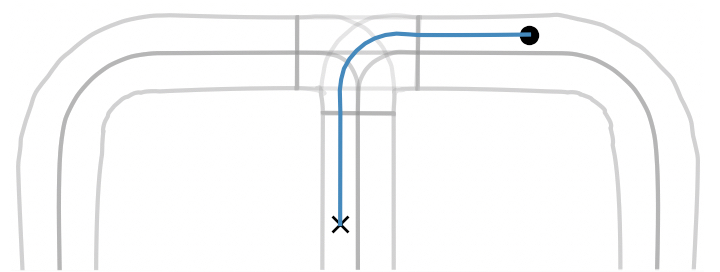
\includegraphics[width=0.3\textwidth]{images/cubetown_1}
    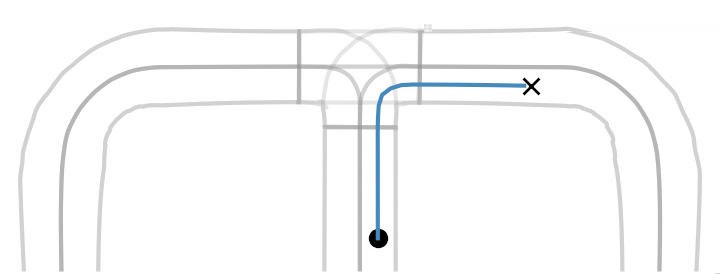
\includegraphics[width=0.3\textwidth]{images/cubetown_2}
    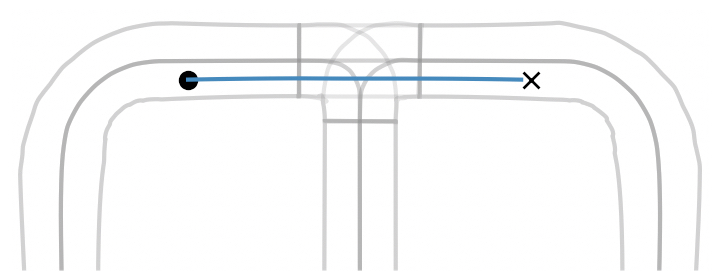
\includegraphics[width=0.3\textwidth]{images/cubetown_3}
  \caption{Sample driving scenarios generated by \tool from an intersection in the Cube Town map available for the \challenge. Driving scenarios begin before entering an intersection~($\bullet$) and end after passing it~($\times$). Top: left turn; Middle: right turn; Bottom: straight through.}
  \label{fig:samples-cubetown}
\end{figure}

Detailed road maps consist of roads composed of lanes, their interconnections (e.g., intersections, junctions), and traffic regulations controlling them (e.g., speed limit, traffic direction); hence, they allow testers to create rich, coherent, and diversified driving scenarios~\cite{althoff2018automatic,bender2014lanelets}. 
%
Among the existing formats to model road maps, in this work, we rely on the notion of \emph{lanelets}~\cite{bender2014lanelets}, an innovative concept for road representation adopted by many (see Section~\ref{subsect:lanelets}).
%
Specifically, we rely on the semantics encoded in the lanelets representation of existing maps to identify intersections and create relevant driving scenarios around and across them. In other words, we abstract existing maps into the lanelets format to generate relevant and diversified \emph{abstract} driving scenarios. Next, we instantiate those abstract scenarios into concrete ones and generate simulation-based test cases that automatically challenge the autonomous vehicle's software in existing driving simulators.

In this paper, we present \tool that implements our approach and summarize its evaluation in the context of the \challenge.
\tool, which is dubbed after the author's first names ---Stephan, Alessio, and Vuong--- and means ``safe'' in Italian, works under the consideration that because manually generated road maps are costly and valuable, testers must use (and re-use) them wisely and extensively. 
Consequently, and in contrast to many existing test case generators (e.g., ~\cite{DBLP:conf/icse/GambiMF19,DBLP:conf/icse/HuynhGF19,DBLP:conf/sigsoft/RiccioT20,DBLP:conf/issta/ZohdinasabRGT21,DBLP:conf/sbst/PanichellaGZR21}) that procedurally generate virtual roads, it leverages existing maps to generate as many tests as possible.
%
However, since generating virtual tests without any guidance is not cost-effective either because not all the generated tests are relevant or because many tests are similar to each other, \tool follows a systematic approach to generate only relevant test cases and maximize their diversity.

The current implementation of \tool takes existing maps in OpenDrive format~\cite{dupuis2010opendrive}, generates abstract driving scenarios involving intersections, and selects among them those that result in quantifiably different ego-vehicle trajectories (see Figure~\ref{fig:samples-cubetown}). Finally, it instantiates the selected scenarios in the industrial driving simulation SVL~Simulator~\cite{rong2020lgsvl} as test cases and automatically executes them.

To promote further research and enable reproducibility of our results, we release \tool as open-source software. \tool's source code and instructions to configure and run it are available at the following link:
\begin{center}
\href{https://github.com/TrackerSB/IEEEAITestChallenge2021}{https://github.com/TrackerSB/IEEEAITestChallenge2021}
\end{center}

\begin{figure}[tp]
  \centering
    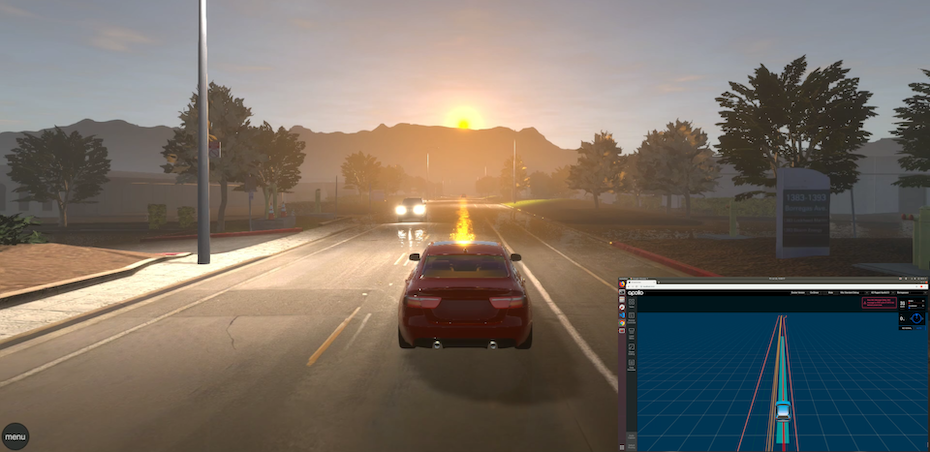
\includegraphics[width=0.5\textwidth]{images/apollo-sim}
  \caption{Apollo Baidu (right, bottom) running with the SVL Simulator~\cite{svl-website}}
  \label{fig:apollosim}
\end{figure}


\section{SVL Simulator}
\label{subsect:lgsvl}
The SVL Simulator~\cite{rong2020lgsvl} is the driving simulation selected for the \challenge.
It is an industrial driving simulator that provides the full simulation stack to test autonomous driving software: On one side, it provides a core simulation engine based on Unity for high fidelity, developer-friendly, cost-effective rigid-body simulation~\cite{craighead2008using}; on the other side, it provides a communication bridge that allows connecting existing autonomous driving stacks such as Autoware~\cite{DBLP:journals/micro/KatoTINTH15} and Apollo Baidu~\cite{apollo}~(see~Figure~\ref{fig:apollosim}). 
Moreover, the SVL Simulator implements additional features such as easily customizing sensors and an API that enables building and managing controllable objects, adjusting the core simulator's modules, and the automated generation and execution of driving scenarios.


\section{Lanelets}
\label{subsect:lanelets}
Lanelets are a novel concept to represent road maps in both topological and geometrical terms. Lanelets models \emph{drivable} road segments and roughly correspond to (segments of) road lanes~\cite{bender2014lanelets}. They are defined by left and right bounds implemented as polylines (i.e., list of points), connected to define complex road maps, and overlapping to form intersections, joins, and merges. Since lanelets encode allowed traffic directions, they help determine the route from a predefined starting point to a given destination~\cite{PekIV20}.

\begin{figure}[tp]
  \centering
    \includegraphics[width=0.5\textwidth]{images/lanelets_01}
  \caption{An example of lanelets \cite{althoff2018automatic}.}
  \label{fig:lanelets}
\end{figure}

As illustrated in Figure~\ref{fig:lanelets}, lanelets can be connected to establish semantic relations that form longer road segments, intersections, merges and joins, and complex road networks. Therefore
they can be used as an intermediate format to represent existing road maps~\cite{althoff2018automatic}. For example, \emph{adjacent} lanelets share one of the two bounds while \emph{preceding/following} lanelets share start or end points in accordance to their traffic direction~\cite{althoff2018automatic}. Notably, lanelets that overlap and share start or end points form intersections~\cite{Althoff2017a}.
%
As we detail later, \tool relies on those features to automatically identify the intersections in existing road maps by analyzing their lanelets representation and define (abstract) driving scenarios across them.


\section{Automatically Generating Diversified Tests from Existing Maps}
This section describes our approach to analyze existing maps and generate sets of diversified driving scenarios using two metrics to establish tests diversity. Instead, the following sections present \tool's evaluation in the context of the \challenge, discuss the achieved results and describe promising ideas for future work.

\begin{figure*}[t]
\minipage{0.33\textwidth}
\includegraphics[width=\linewidth]{images/distance_cubetown_2}
\endminipage\hfill
\minipage{0.33\textwidth}
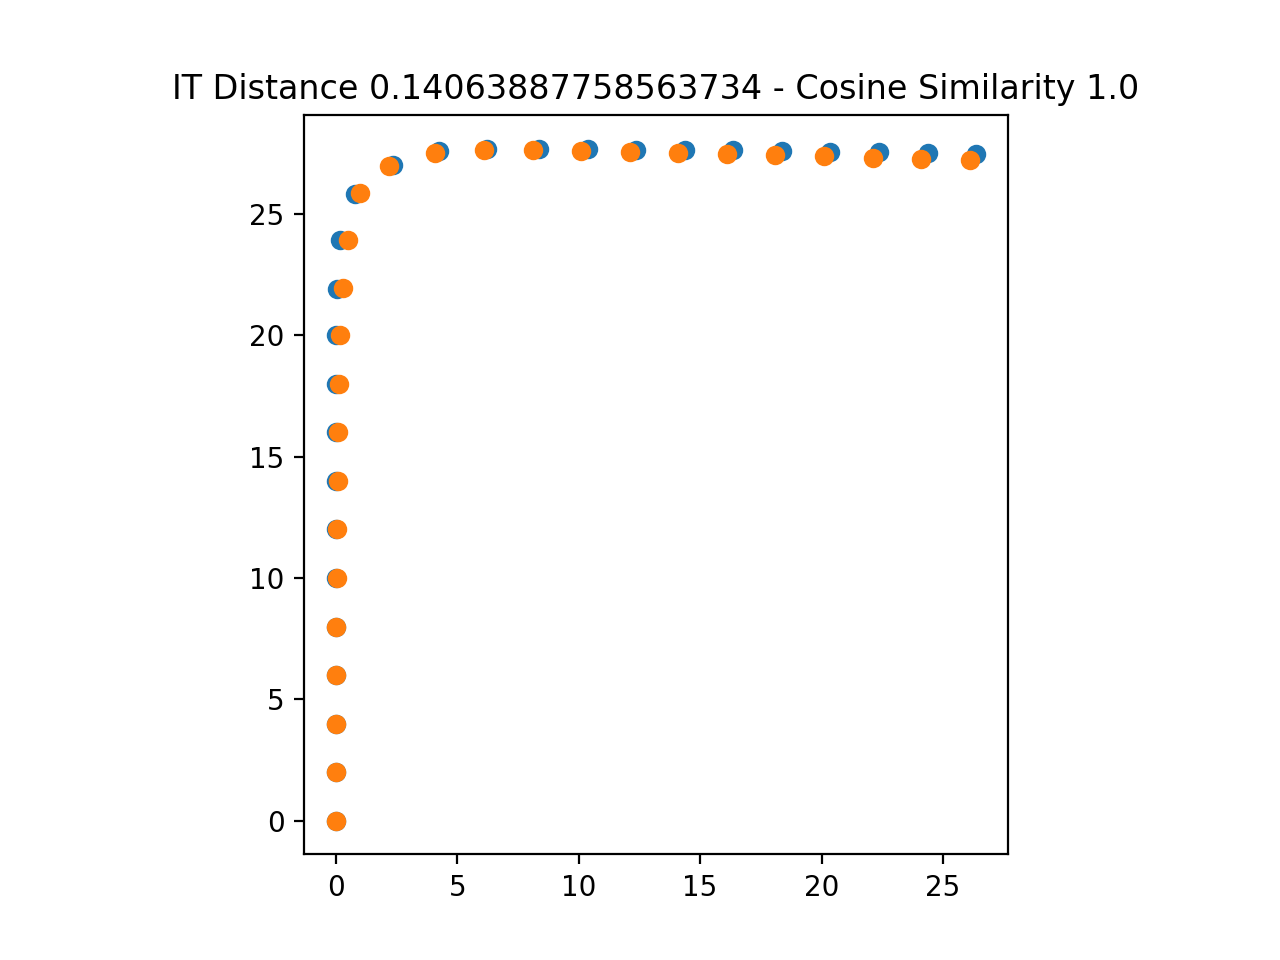
\includegraphics[width=\linewidth]{images/distance_cubetown_1}
\endminipage\hfill
\minipage{0.33\textwidth}%
  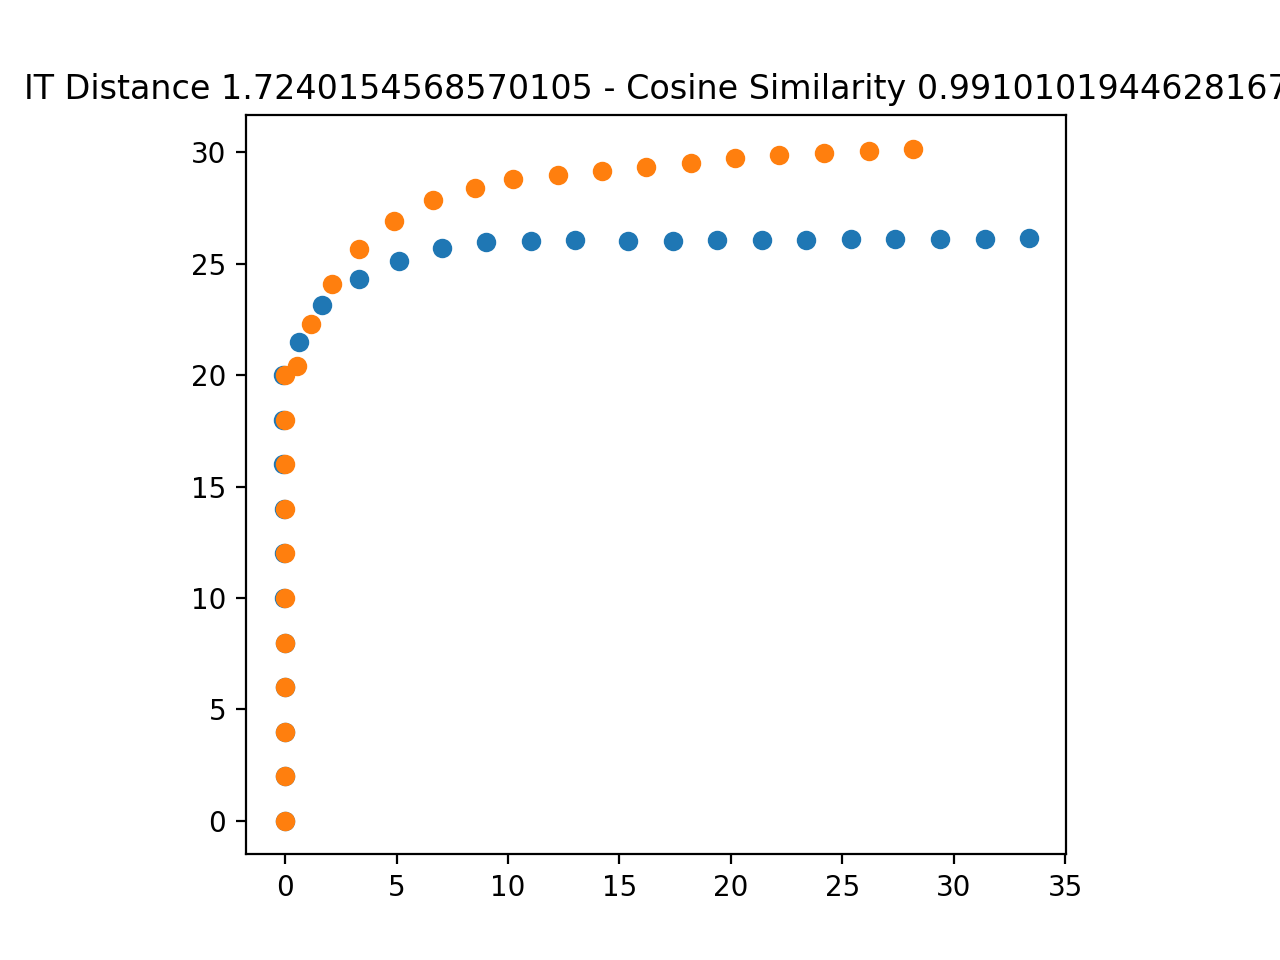
\includegraphics[width=\linewidth]{images/distance_ba_2}
\endminipage
\caption{Examples of similar trajectories. In each plot, we compare pairs of trajectories generated by \tool and report their similarity computed using standard metrics such as the iterative Levenshtein distance (IT~Distance) and Cosine similarity. For example, the first two plots result from the Cube Town map and illustrate cases of very similar roads, while the rightmost plot, which results from the Borregas Avenue map, shows partially overlapping trajectories.}
\label{fig:similarity}
\end{figure*}


\subsection{\tool in a Nutshell}
\tool is entirely automatic and can generate test cases that stress the ego-vehicle in many different ways, possibly involving static obstacles that partially or completely occlude the lane in which the ego-vehicle is driving. 

Given a map in OpenDrive format \tool \begin{inparaenum}[(1)]
\item identifies the intersections the map contains, 
\item generates abstract driving scenarios that force the ego-vehicle to plan trajectories to cross those intersections safely, \item selects abstract driving scenarios that maximize the diversity of the allegedly planned trajectories, and \item generates executable test cases implementing the selected abstract driving scenarios.
\end{inparaenum}

\tool can also extend the set of generated test cases by reusing existing ones and placing static obstacles, i.e., Non-Playable Characters (NPC) vehicles, in the lane occupied by the ego-vehicle. By doing so \tool achieves two secondary goals: first, it further increases the diversity of the generated tests, as the obstacles force the ego-vehicle to plan new trajectories; second, it allows testing the ego-vehicle's object detection and collision avoidance in addition to route planning and lane-keeping.

The following sections detail each step of the proposed approach.

\subsection{Identifying Intersections}

\begin{figure}
  \centering
    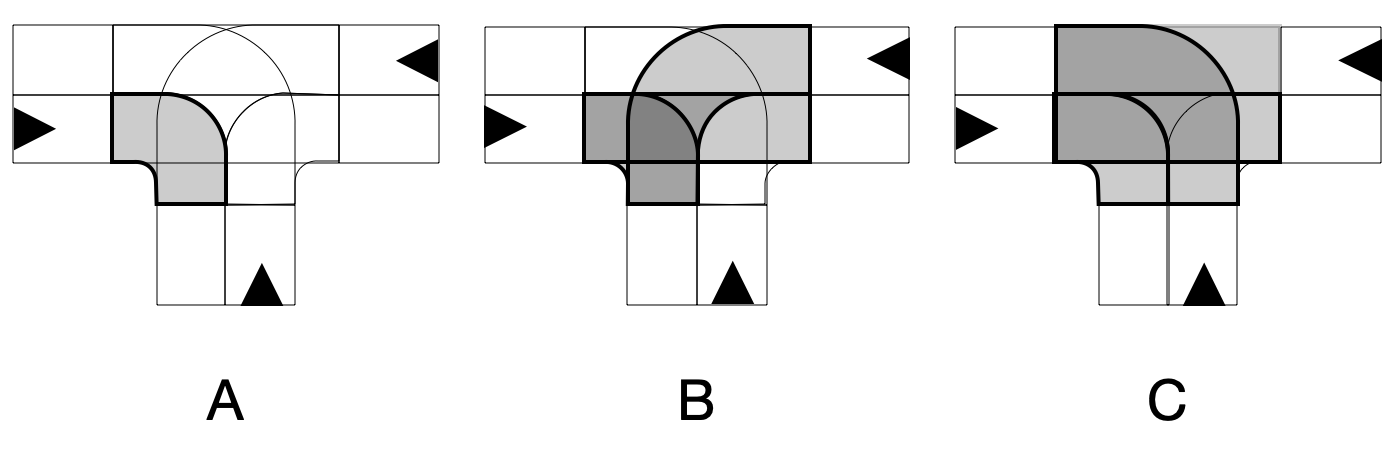
\includegraphics[width=0.95\columnwidth]{images/overlapping}
  \caption{An example of an intersection constructed by \tool by transitively identifying overlapping lanelets.}
  \label{fig:overlapping}
\end{figure}

\tool uses the opendrive2lanelet library~\cite{althoff2018automatic} to translate the original maps from the OpenDrive format to the lanelets format. As discussed in Section~\ref{subsect:lanelets}, lanelets are connected by relations like `follow` and `adjacent` that define their semantics and provide geometrical information (e.g., their shape). 
However, since the lanelets format lacks a standardized way to capture intersections explicitly, i.e., via formalized relations between lanelets, \tool implements a heuristic to identify them: 
First, it uses geometric information about lanelets to identify overlapping lanelets (\mbox{Figure~\ref{fig:overlapping}-A} and \mbox{Figure~\ref{fig:overlapping}-B}) as they are likely to belong to the same intersection. Second, since not all the lanelets in the same intersection directly overlap with each other, \tool groups together lanelets that \emph{transitively} overlap (\mbox{Figure~\ref{fig:overlapping}-C}).


\begin{figure}
  \centering
    \includegraphics[width=0.95\columnwidth]{images/nonoverlapping}
  \caption{An example of an intersection constructed by \tool by exploiting the relationships among lanelets.}
  \label{fig:nonoverlapping}
\end{figure}

The intersections identified this way may be incomplete because, in some cases, lanelets that logically should belong together do not overlap with the other lanelets already assigned to those intersections. The bolded lanelets in Figure~\ref{fig:nonoverlapping} exemplify two instances of this situation. \tool identifies those missing lanelets by leveraging the relations defining the lanelet network. For example, for the case reported in \mbox{Figure~\ref{fig:nonoverlapping}-A} \tool includes in the intersection Lanelet~$1$ because it is adjacent to a lanelet already assigned to that intersection, i.e., Lanelet~$2$. For the case reported in \mbox{Figure~\ref{fig:nonoverlapping}-B}, instead, \tool includes Lanelet~$1$ because it precedes Lanelet~$2$ that is adjacent to Lanelet~$3$, the successors of a lanelet already assigned to that intersection, i.e., Lanelet~$4$. 
%
Noticeably, the heuristic implemented by \tool to identify intersections exploiting the relations between lanelets and without user input is different from the one proposed by Klischat et al.~\cite{DBLP:conf/itsc/KlischatLHA20} that instead relies on hierarchical clustering and requires the user to specify a minimum size for the intersection.

After identifying the intersections in the map, \tool can generate driving scenarios that force the ego-vehicle to cross them.

\subsection{Generating Relevant Scenarios}
\tool generates abstract driving scenarios that follow legal trajectories across intersections such as those reported in Figure~\ref{fig:samples-cubetown}. We define those trajectories as legal because they follow the traffic directions encoded into the lanelets. Additionally, we limit \tool to consider only the simplest form of such trajectories, i.e., those that do not require the ego-vehicle to switch lanes. Therefore, a typical driving scenario generated by \tool starts on a lane \emph{before} an intersection, continues on the same lane across that intersection, and finally ends on the (logically) same lane \emph{after} that intersection.
%
\begin{figure}
 \centering
  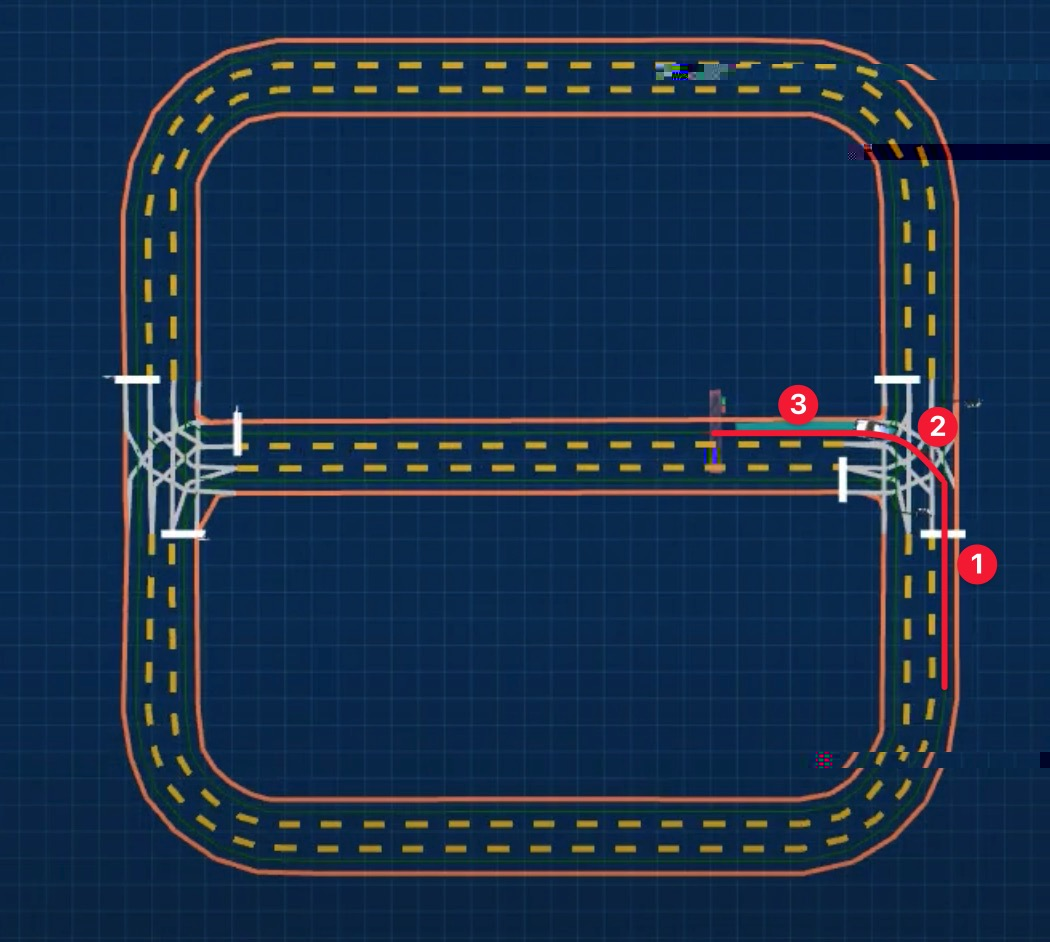
\includegraphics[width=\columnwidth]{images/lanelet01}
 \caption{An example of an abstract driving scenario generated by \tool in the Cube Town map. The scenario  starts on a lane~(1), continues inside the intersection by following the lane~(2), and ends on the same lane after passing the intersection (3).}
 \label{fig:intersection_sf}
\end{figure}

\tool generates driving scenarios by selecting the lanelets that belong to an intersection (Figure~\ref{fig:intersection_sf}) and then including those lanelets outside the intersection that precede and follow the selected ones. Notably, because intersections have various configurations (e.g., number of entering and exiting lanes), the generated driving scenarios can stress different behaviors of ego-vehicle by forcing it to turn left, turn right, or go straight through the intersection.

The generated scenarios are composed of the smallest number (i.e., three) of lanelets. This feature arguably increases the understandability of the resulting test cases but does not necessarily guarantee fast test executions. For example, the lanelets preceding or following an intersection may be long, requiring some time to be fully traversed during test execution. Therefore, to reduce execution time, \tool places the ego-vehicle at a fixed distance before entering the intersection and sets the target position to reach at a fixed distance after passing the intersection. Because those distances are configurable, testers can control the duration of test executions and enable the generation of tests involving obstacles (see~Section~\ref{sec:spicing-up}).


\subsection{Selecting Diversified Scenarios}
Up to this point, \tool does not take the diversity of scenarios into account as it simply generates as many scenarios as possible to explore the possibilities offered by the input road map. However, many legal trajectories may stress the ego-vehicle similarly; for example, they may force it to drive straight through the same intersections from multiple directions. Therefore, \tool filters out test cases that are too similar to each other to improve testing cost-efficiency.
%
We experimented with two (greedy) approaches for filtering out test cases based on distance metrics and feature maps.

\subsubsection{Filtering Similar Scenarios by Similarity}
The first approach to select diversified scenarios relies on the similarity between the trajectories imposed by the driving scenarios on ego-vehicle. After an initial exploration considering standard metrics such as edit distance and cosine similarity (see~Figure~\ref{fig:similarity}), we decided to adopt the Levenshtein distance to quantify the similarity of generated scenarios. The Levenshtein distance quantifies the similarity between trajectories by measuring how many \emph{edits} are required to transform one trajectory into the other; the smaller the number of edits is, the more similar the two trajectories are. Notably, \tool can use the Levenshtein distance because we represent trajectories as coordinates arrays, and edits correspond to insertions, deletions, and substitutions of arrays' entries. Specifically, \tool calculates the Levenshtein distance between pairs of trajectories using the code provided by DeepJanus~\cite{DBLP:conf/sigsoft/RiccioT20} and discards all the driving scenarios whose trajectories are too similar to the trajectories of driving scenarios already selected. 
%
Testers can control the similarity between the trajectories using a configurable threshold to create larger or smaller test suites. For completeness, in our evaluation we filtered out trajectories with a distance value smaller than $1.9$.

%A similar approach to select diverse trajectories was followed by Zohdinasab and co-author in a pilot study to identify road features relevant for testing lane keeping systems~\cite{DBLP:conf/issta/ZohdinasabRGT21}.
%As \tool, they took inspiration for the computation of the iterative Levenshtein distance from the work of Riccio and Tonella~\cite{DBLP:conf/sigsoft/RiccioT20}.

\subsubsection{Filtering Driving Scenarios using Feature Maps}
The second approach to select diversified scenarios utilizes the feature maps defined by Zohdinasab et al.~\cite{DBLP:conf/issta/ZohdinasabRGT21}. 
Trajectory features capture high-level characteristics of the abstract scenarios that are relevant for testing self-driving car software; examples of those features are the number of turns and the minimum curvature\footnote{The minimum curvature highlights the presence of sharp turns.} that quantify how difficult it would be to follow the trajectory. Instead, feature maps place driving scenarios in a two-dimensional space according to the values taken by their features and provide a compact and understandable representation of their most salient aspects. Intuitively, scenarios with similar features are placed in nearby cells, whereas scenarios that are far away in the map have very different features (see Figure~\ref{fig:feature-maps}).

\begin{figure*}[t]
\minipage{0.33\textwidth}
\includegraphics[width=\linewidth]{images/feature_cubetown}
\endminipage\hfill
\minipage{0.33\textwidth}
\includegraphics[width=\linewidth]{images/two_roads_same_cell.png}
\endminipage\hfill
\minipage{0.33\textwidth}%
  \includegraphics[width=\linewidth]{images/roads_different_cell.png}
\endminipage
\caption{Examples of feature map and trajectories for the Cube Town map. 
Left panel: The feature map generated by \tool using direction coverage (dc) and minimum radius (mr) as features.
Central panel: Similar trajectories sampled from the same cell in the feature map, i.e., $(6,1)$.  
Right panel: Diverse trajectories sampled from distant cells in the feature map, i.e., $(10,2), (1,10), (6,1)$.}
\label{fig:feature-maps}
\end{figure*}

\tool's goal is to generate driving scenarios that result in trajectories with different characteristics; therefore, given a feature map filled with all the generated trajectories, \tool selects from each cell at most one trajectory (i.e., driving scenario) as the representative for the class of trajectories with the same feature combination while discarding the others.

Notably, using the feature maps, testers can easily quantify the coverage achieved by \tool by counting the number of cells that contain at least one driving scenario. Likewise, content generators can use the feature maps to assess the ``richness'' of the road maps. 
%
For example, figures~\ref{fig:feature-maps-cubetown}~--~\ref{fig:feature-maps-sanfrancisco} show the road map (top plot) and the corresponding feature map (bottom plot) for the five maps we used in the \challenge (see Section~\ref{sec:evaluation}). From those figures, we can make the following observations: 
\begin{inparaenum}[(1)]
\item road maps of increasing complexity, i.e., maps that contain more intersections, result in feature maps that are more covered, 
and \item road maps with a repetitive structure result in feature maps with very dark cells, i.e., cells that contain many trajectories with very similar features.
\end{inparaenum}


\subsection{Generating Test Cases}
\tool defines abstract driving scenarios as combinations of lanelets. So it needs to concretize them into executable test cases featuring test oracles that check if the ego-vehicle reaches the target location and if it does so within a predefined timeout. Also, \tool must configure the driving simulation to place the ego-vehicle in the starting position and rotate it according to the road direction. However, doing so may not be enough to ensure that the generated tests are reliable and reproducible because the simulations include additional components with randomized behaviors that can affect the test results. For example, if the ego-vehicle needs to pass an intersection controlled by a traffic light, its state affects the behavior of the ego-vehicle: if the traffic light is red, the ego-vehicle must stop before it, which may cause the timeout to trigger a false positive. However, executing multiple times the same test may produce different results, hence flakiness, as the traffic light's initial state is initialized at random unless configured explicitly by the test. Therefore, to avoid false positives and reduce test flakiness, \tool programs the traffic lights on the expected trajectories to turn green when the ego-vehicle approaches them.

\subsection{Spicing Up the Test Cases}
\label{sec:spicing-up}
The tests generated by \tool are diverse but plain: they stress the ability of the ego-vehicle to plan various trajectories to pass the intersections while keeping the lane but involve no other elements besides the ego-vehicle and the traffic lights. To further increase the diversity of the generated tests and enable testing additional features of the ego-vehicle such as object detection and collision avoidance, we let \tool extend the basic tests by placing static obstacles, i.e., NPC vehicles, on the course of the ego-vehicle.

Our approach to ``spice up'' tests consists in placing an NPC vehicle in predefined positions between the ego-vehicle's initial position (i.e., the starting point of the driving scenario) and the intersection to pass such that the NPC vehicle partially or entirely occludes the lane that the ego-vehicles is supposed to keep. Default occlusions are partial and cause the ego-vehicle to swerve before entering the intersection; \tool can place the NPC vehicle either on the left or right side of the lane, but not both. Additionally, but only if the geometry of the intersection allows it, \tool can place the NPC in the middle of the lane in front of the ego-vehicle, forcing it to switch lanes before entering the intersection.

In summary, on top of the diversified test cases that \tool generates from a given map, testers can quickly generate up to four times more test cases by simply letting \tool add NPC vehicles in front of the ego-vehicle. Notably, we limit \tool to place a single NPC vehicle per test case to keep them as simple and understandable as possible.

\subsection{Prototype}
We implemented \tool in Python (v3.9) as a command-line application and integrated it with the SVL driving simulator (v2021.01) in accordance to the rules of the \challenge.
For the evaluation, we ran \tool on a gaming laptop running Ubuntu~20.04.2~LTS, the SVL driving Simulator, and Apollo Baidu (v6.0).

\section{Evaluation}
\label{sec:evaluation}

\subsection{Experimental Settings}
We evaluated \tool according to the main objectives defined in the \challenge, i.e., generation of diverse tests, automated test generation and execution, and generation of tests that can find problems in Apollo Baidu, and the (limited) resources we had at the time the \challenge took place.

Since we deem the first two objectives more relevant than the last one, we devoted more effort to address them. Consequently, we evaluated the ability of \tool to generate diverse and executable test cases automatically using various maps available for the SVL Simulator, but run the tests against Apollo Baidu only for one map.

As summarized in Table~\ref{tab:results-generation}, we selected five maps of increasing size (see figures~\ref{fig:feature-maps-cubetown}~--~\ref{fig:feature-maps-sanfrancisco}) and complexity (see column \emph{Intersections} in Table~\ref{tab:results-generation}). Our selection was limited by the availability of the maps and their compatibility with the opendrive2lanelets library. 
%
As summarized in Table~\ref{tab:results-effectiveness}, we tested Apollo Baidu only on the Cube Town map with all the test cases generated from the plain scenarios selected using similarity and feature maps (columns \emph{Plain}) and some test cases generated by placing NPC vehicles (columns \emph{NPC}). Specifically, we created the NPC tests by randomly sampling three selected scenarios from each set and placing the NPC vehicle on the ego-vehicle's left, right, and front. The table reports the number of failed test cases followed by the number of total tests executed.



\subsection{Achieved Results}

\begin{table}[t]
    \centering
      \caption{\tool's Evaluation Results: Test Generation and Selection}
      \label{tab:results-generation}
      \begin{tabular}{lrrrr}
        \toprule
        \multicolumn{1}{c}{\textbf{Map Name}}&
        \multicolumn{1}{c}{\textbf{Intersections}}&
        \multicolumn{3}{c}{\textbf{Test Cases}}\\ \cmidrule(lr){3-5}
        & & Total & Similarity & Feature Map\\
        \midrule
        Cube Town & 2 & 12 & 8 & 5\\
        Borregas Ave & 2 & 28 & 20 & 16\\
        Shalun & 14 & 149 & 124 & 33\\
        Gomentum & 25 & 126 & 110 & 25\\
        San Francisco & 89 & 806 & 535 & 52\\
        \midrule 
        \textbf{Total} & 132 & 1121 & 797 & 131\\
        \bottomrule
      \end{tabular}
\end{table}

As reported in Table~\ref{tab:results-generation}, \tool identified more than a hundred intersections and generated more than a thousand driving scenarios that do not involve NPC vehicles. From those scenarios, it selected between 7\% (San Francisco) and 57\% (Borregas Ave) scenarios for the execution using features maps, whereas using similarity, it selected considerably more cases (up to 87\% for Gomentum).

These results suggest that \tool could handle maps of considerable size and effectively identify intersections in them. Furthermore, regarding test generation, it was able to identify many driving scenarios and selected among them different driving scenarios. The results also suggest that feature maps may be more stringent in selecting test cases than similarity computed using edit distance. However, this observation should be taken with care, as the number of selected test cases using feature maps depends on their configurations, i.e., the selected features and their granularity.

\begin{table}[t]
    \centering
      \caption{\tool's Evaluation Results: Test Effectiveness}
      \label{tab:results-effectiveness}
      \begin{tabular}{l rr rr}
        \toprule
        \multicolumn{1}{c}{\textbf{Map Name}} &
        \multicolumn{2}{c}{\textbf{Similarity}} & % \cmidrule(lr){3-5}
	\multicolumn{2}{c}{\textbf{Feature Map}}\\ \cmidrule(lr){2-3}\cmidrule(lr){4-5}
        & Plain & NPC & Plain & NPC \\
        \midrule
        Cube Town  & 3/8 & 1/3 & 0/5 & 1/3\\
        \bottomrule
      \end{tabular}
\end{table}

As reported in Table~\ref{tab:results-effectiveness}, the execution of the generated test cases resulted in some failed test cases despite the simplicity of the map. Noticeably, all the failures are caused by the test subject not reaching the target location in time, meaning that the ego-vehicle did not crash into the NPC vehicles nor left the lane but could not plan or execute a suitable trajectory. 

Regarding plain tests, we can observe that selecting tests using similarity resulted in more failures than selecting tests using the feature map. Instead, regarding NPC tests, we can observe that one test failed consistently in both configurations. Upon manual inspection of the failed tests, we noticed that the NPC vehicle was always parked in the middle of the ego-vehicle's lane. This observation suggests either the ego-vehicle failed to plan a trajectory that required to switch the lane or that, although we took extra care to remove possible causes of false positives (e.g., traffic lights, the minimal distance of the NPC car from the intersection), we may have missed something. For example, we may have oversight the possibility that ego-vehicle cannot invade the opposite traffic direction to pass the obstacle, forcing it to wait behind the obstacle indefinitely.

\begin{figure*}[!tp]
\hfill
\minipage{0.33\textwidth}
  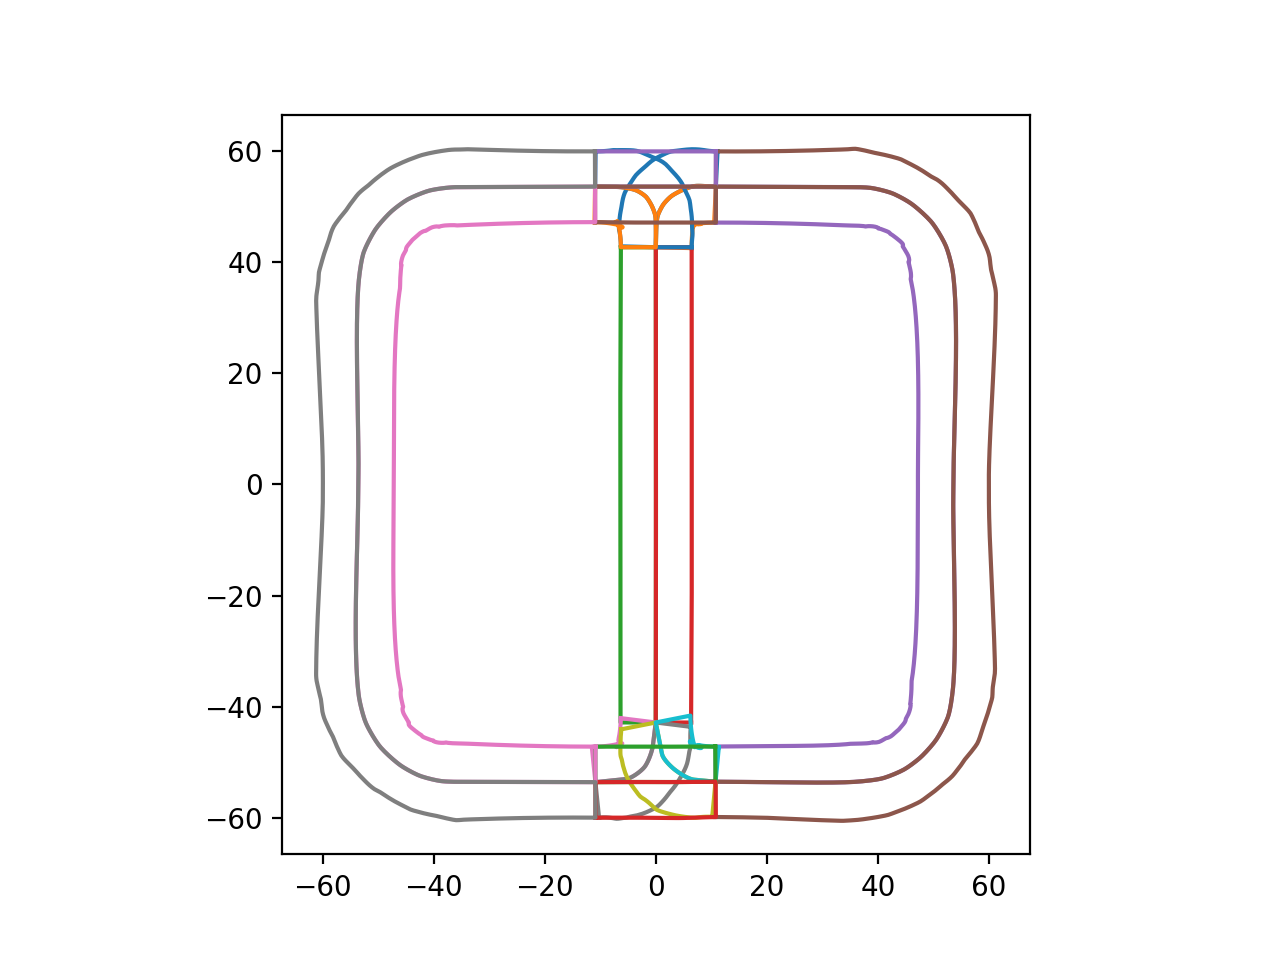
\includegraphics[width=\linewidth]{images/map_cubetown}
  \includegraphics[width=\linewidth]{images/feature_cubetown}
  \caption{Cube Town map.}
  \label{fig:feature-maps-cubetown}
\endminipage\hfill
\minipage{0.33\textwidth}
  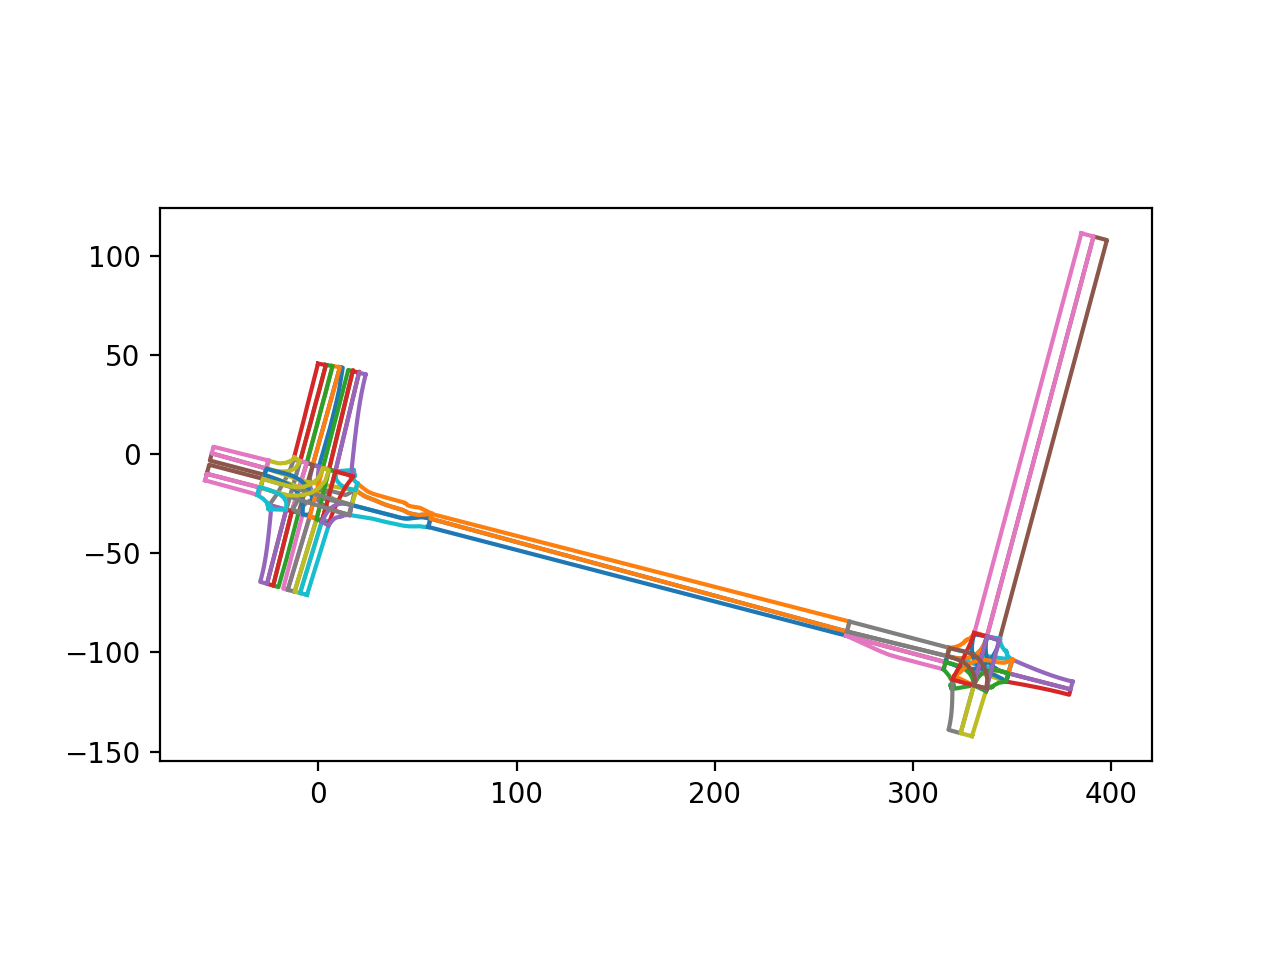
\includegraphics[width=\linewidth]{images/map_borregasave}
  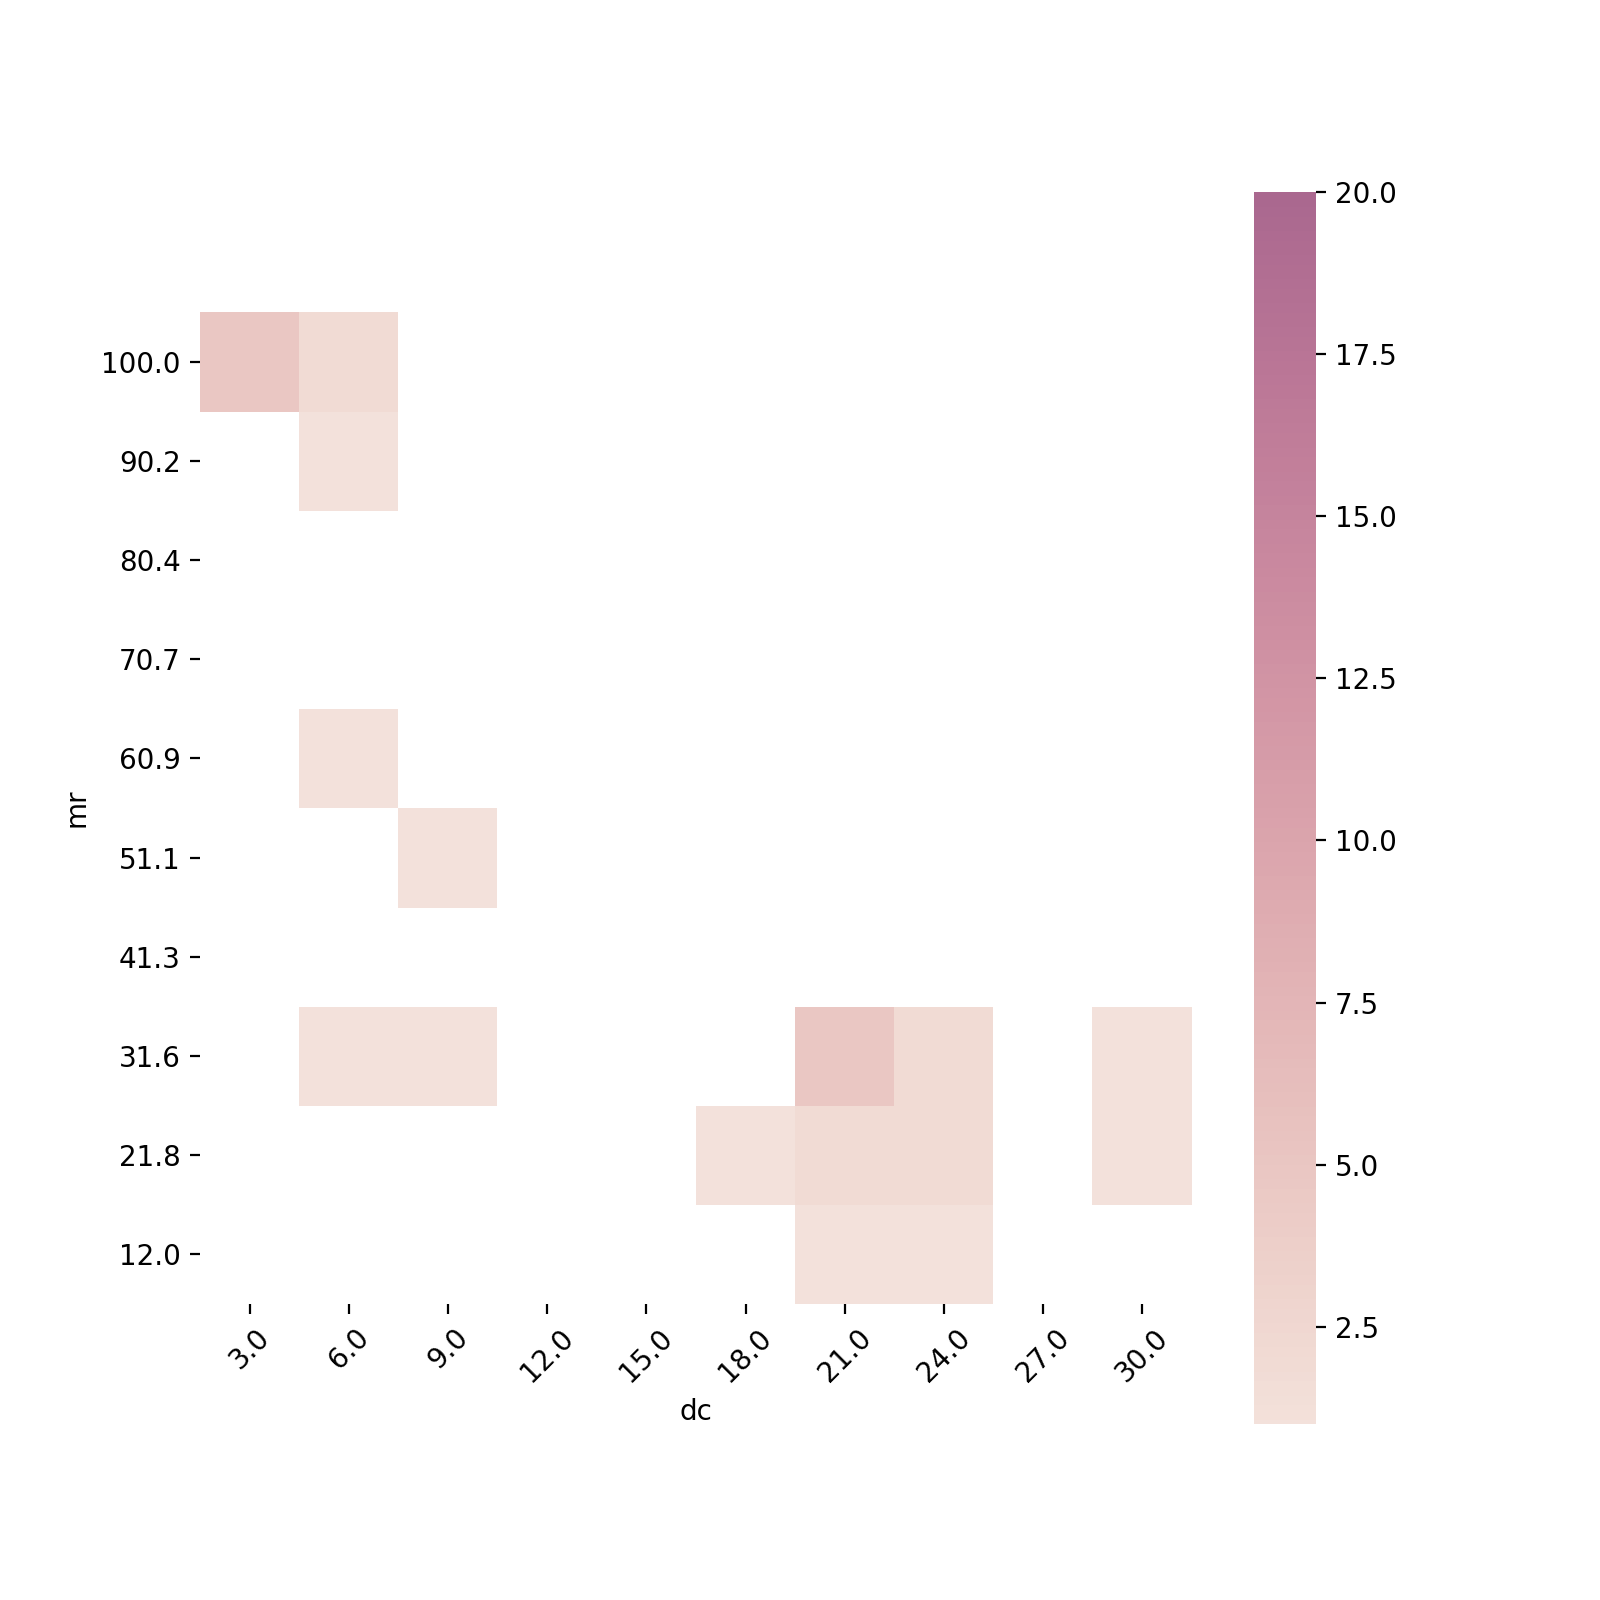
\includegraphics[width=\linewidth]{images/feature_borregasave}
  \caption{Borregas Ave map.}
    \label{fig:feature-maps-borregas}
\endminipage\hfill
\minipage{0.33\textwidth}%
  \includegraphics[width=\linewidth]{images/map_shalun}
  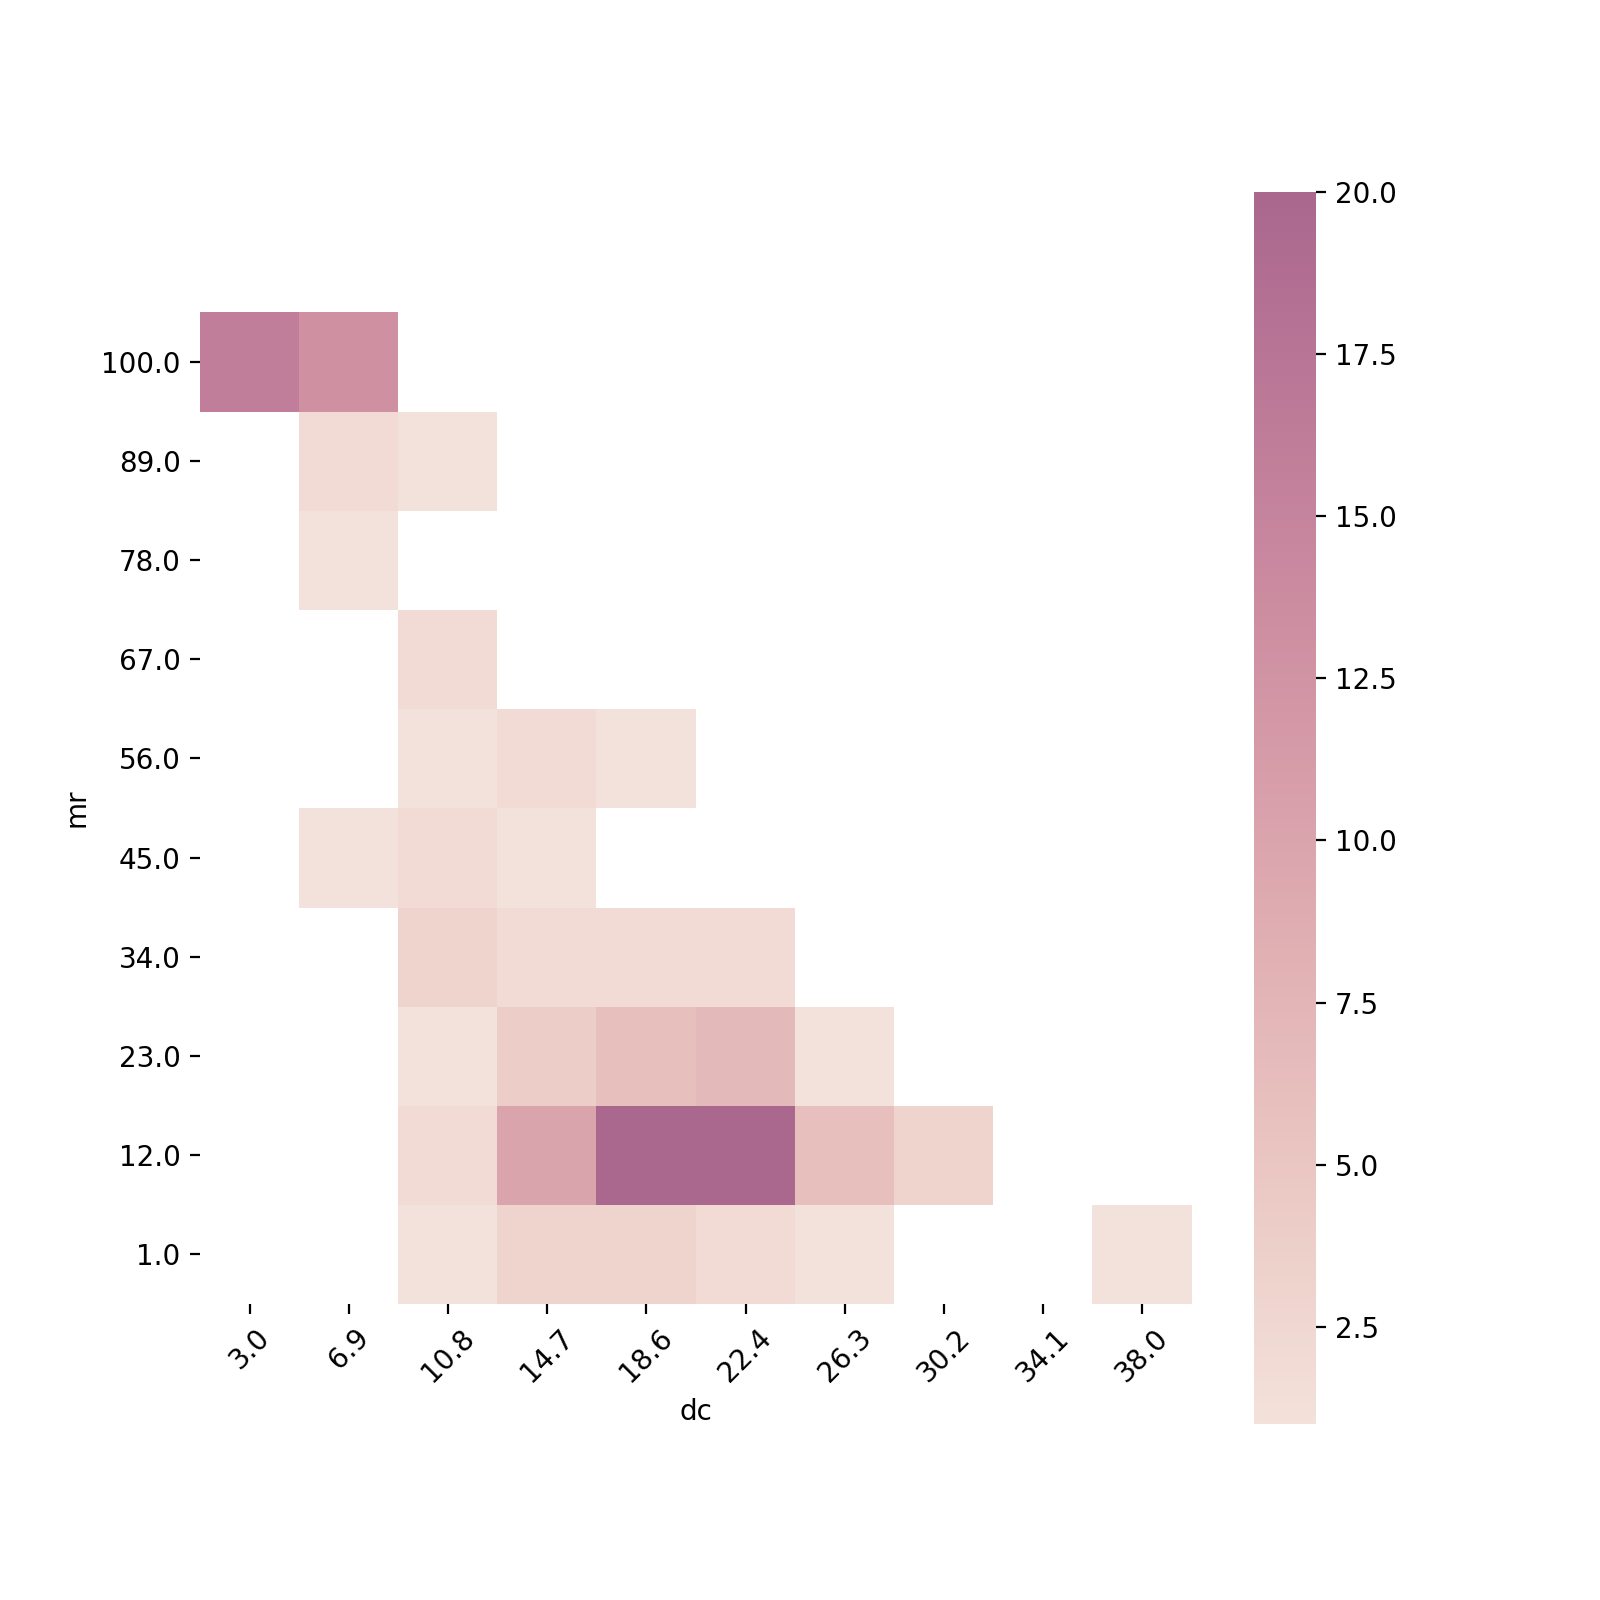
\includegraphics[width=\linewidth]{images/feature_shalun}
  \caption{Shalun map.}
    \label{fig:feature-maps-shalun}
\endminipage 
\hfill
\end{figure*}

\begin{figure*}[p]
\minipage{0.33\textwidth}%
  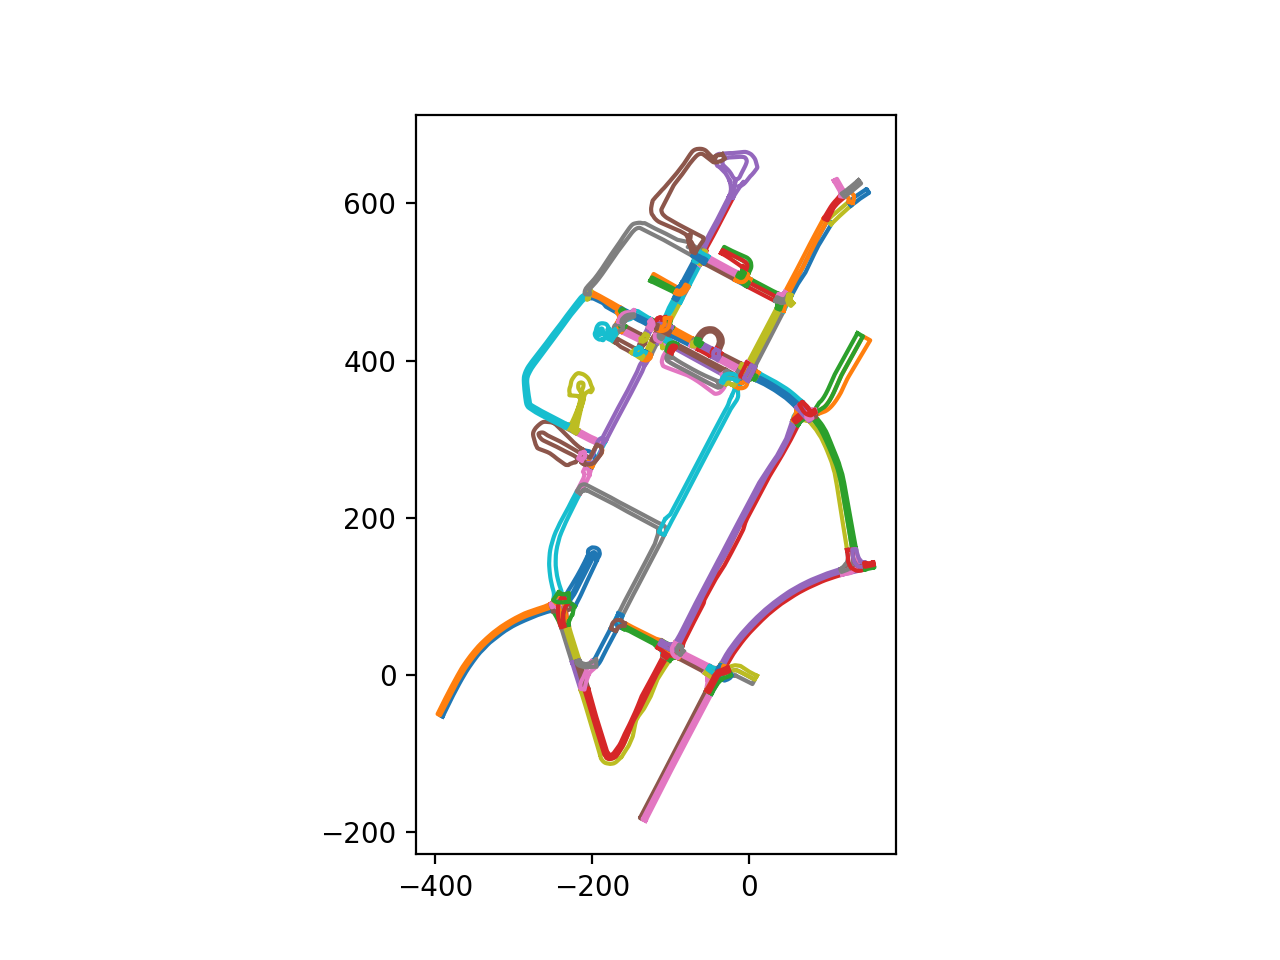
\includegraphics[width=\linewidth]{images/map_gomentum}
  \includegraphics[width=\linewidth]{images/feature_gomentum}
  \caption{Gomentum map.}
    \label{fig:feature-maps-gomentum}
\endminipage\hfill
\minipage{0.33\textwidth}%
  \includegraphics[width=\linewidth]{images/map_sanfrancisco.png}
  \includegraphics[width=\linewidth]{images/feature_sanfrancisco.png}
  \caption{San Francisco map.}
    \label{fig:feature-maps-sanfrancisco}
\endminipage
\hfill
\end{figure*}

\section{Future Work}

In the hope of capturing the intended aim of the challenge, we brainstormed possible ideas to implement for future work. We tried to ``think out-of-the-box'' while remaining pragmatic. Below we summarize two of such ideas.

\paragraph{Parking Lot Madness}
Create scenarios that take place inside parking lots to test features like ``Smart Summon.'' The idea is to check if the ego-vehicle can safely drive from a parking spot to the parking lot's exit despite pedestrians and other vehicles. Our vision is to generate scenarios by placing the ego-vehicle in different parking spots and controlling the placement and movement of NPC cars and pedestrians to create various critical situations.

\paragraph{To Pass or Not to Pass?}
Check the behavior of the ego-vehicle while handling controlled intersections. 
The idea is to take any map, find where controlled intersections and traffic lights are, and (automatically) generate scenarios where the car must pass the various controlled intersections, possibly "trapping`` the ego-vehicle in the middle of them by directly acting upon the traffic lights (e.g., flashing lights, turn lights off).
%
%Concrete tests can be generated by changing which controlled intersection to pass, the direction that ego-vehicle should follow (e.g., turn right, go straight), and directly acting upon the traffic lights (e.g., flashing lights, turn lights off).
%
%Alternatively, we can also place the ego-vehicle in the middle of controlled intersections and try to ``trap it there'' by controlling the traffic lights. This additional arrangement will let us check whether the vehicle can adequately free the controlled intersections or get stuck in the middle of them.

% References
\bibliographystyle{IEEEtran}
\bibliography{biblio}

\end{document}
